\section{Numerical Experiments}\label{sec:numerical-experiments}

Throughout this section we present some numerical experiments. These were selected from the \href{changedetection.net}{changedetection.net} datasets. Our procedure works as follows: While reading the data stream of images we normalise every image vector by its norm, such that $\norm{\bl{f}_k}{2} = 1$ holds for all input data. This data normalisation is useful in DMD because the scaling of the data directly influences the numerical computations and thus the quality of the returned quantities~\cite{Drmac2020}. Afterwards, we perform QR compressed streaming DMD as explained in Algorithm~\ref{alg:qr-streaming-dmd} on the incoming data. In a first run we plot the minimal values of all dynamic residuals for a small number of data snapshots to decide upon a cut-off tolerance for background and motion detection. Once this threshold has been chosen, we compute the background reconstructions and foreground masks as explained in Section~\ref{sec:motion-detection}. We repeat this process for a select number of parameter combinations, mostly varying the size of the data memory $\ell_\text{mem}$. Our experiments show that in the streaming setting even a small number of stored snapshots and a low reconstruction/truncation rank suffice to provide good foreground masks.

All code used to generate the results of this report has been uploaded to \href{https://github.com/peoe/dmd-math-656/}{github.com/peoe/dmd-math-656/}. Included in this repository are a setup file for the Python environment required, as well as a script to aid in acquiring the relevant datasets.

\subsection{Detection of Pedestrians}\label{subsec:pedestrians} % MARK: PEDESTRIANS

The pedestrian dataset obtained from \href{changedetection.net}{changedetection.net} shows a section of a street with pedestrians and a bicyclist passing along the road. This example is a nice benchmark problem because the video contains both a stationary and not very noisy background, but it also includes different movement speeds.

We run both the motion detection and the foreground/background separation algorithm in the streaming DMD setting with a limited snapshot memory size of $\ell_\text{mem} \in \set{5, 10, 15, 20}$. For the foreground/background separation we consider the minimal residuals of the first $100$ frames to determine the residual tolerance $\rho > 0$, see Figure~\ref{fig:pedestrian-exp-residual} for a plot of these first residuals. Afterwards, we compute the separated foreground data with tolerances of $\rho \in \set{8 \cdot 10^{-3}, 5 \cdot 10^{-3}, 3 \cdot 10^{-3}, 10^{-3}}$ for the respective $\ell_\text{mem}$ snapshot memory size. We can see that the minimal residual for every memory size decreases initially as the memory slowly gets filled with snapshots. Then we enter a plateau phase where the minimal residual remains consistently small before increasing after $i = 50$ where the first pedestrian enters the frame. Noticably, the minimal residual for larger memory sizes spikes to a large number as soon as the scene changes upon the entrance of a moving foreground object. This is due to the fact that at this point the snapshot memory contains a larger number of snapshots do not contain the pedestrian, and hence the dynamic modes mostly reconstruct the static background instead of the moving foreground. This can be mitigated by choosing either a smaller memory size $\ell_\text{mem}$, or by dynamically reducing the length of the memory once we detect a spike in the minimal residual.

\begin{figure}[!ht]
    \centering
    \begin{tikzpicture}
        \pgfplotsset{
            width=16cm,
            height=7cm
        }
        \begin{axis}[
            xmin=0, xmax=100,
            ymin=1e-4, ymax=1e0,
            ymode=log,
            xlabel={Index $i$},
            ylabel={Residual $r_i$},
            legend style={
                at={(0.975, 0.05)},
                anchor=south east,
                legend columns=1,
            }
        ]
            \addplot[color=red, smooth, thick] table[col sep=comma, header=has colnames, x index={0}, y index={1}] {pedestrian_motion_res.csv}; \addlegendentry{$\ell_\text{mem} = 5$}
            \addplot[color=blue, smooth, thick] table[col sep=comma, header=has colnames, x index={0}, y index={2}] {pedestrian_motion_res.csv}; \addlegendentry{$\ell_\text{mem} = 10$}
            \addplot[color=orange, smooth, thick] table[col sep=comma, header=has colnames, x index={0}, y index={3}] {pedestrian_motion_res.csv}; \addlegendentry{$\ell_\text{mem} = 15$}
            \addplot[color=black, smooth, thick] table[col sep=comma, header=has colnames, x index={0}, y index={4}] {pedestrian_motion_res.csv}; \addlegendentry{$\ell_\text{mem} = 20$}
        \end{axis}
    \end{tikzpicture}
    \caption{Residuals $r_i$ for the pedestrian dataset for memory sizes $\ell_\text{mem} \in \set{5, 10, 15, 20}$; In colour: residuals as computed during the streaming algorithm.}\label{fig:pedestrian-exp-residual}
\end{figure}

For selecting the motion or foreground masks we determine an error threshold and select all pixels for which the dynamic background differs from the incoming data by more than the threshold. A comparison of the true image, the computed motion mask, and the foreground mask at frame number $100$ can be seen in Figure~\ref{fig:pedestrian-frame-100}. Notice that the motion mask highlights only the outline of the pedestrian --- as described above this occurs because the dynamic backgrounds in the motion detection procedure only store local information, and thus only detect the movement along object and texture boundaries.

\begin{figure}[!ht]
    \centering
    \begin{subfigure}{.3\textwidth}
        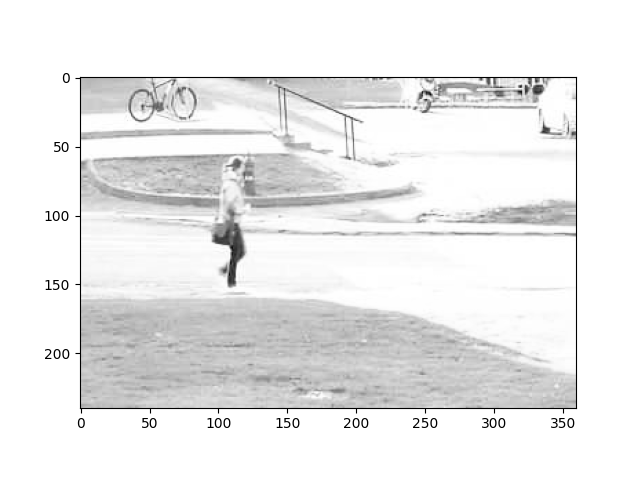
\includegraphics[width=\textwidth]{pedestrian_frame_100.png}
        \caption{True image}
    \end{subfigure}
    \hfill
    \begin{subfigure}{.3\textwidth}
        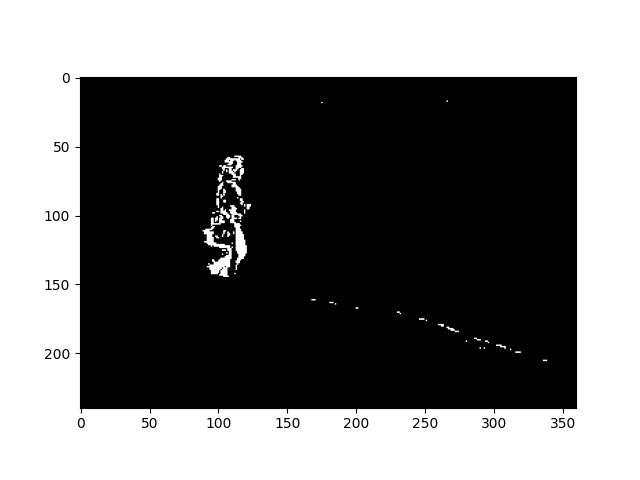
\includegraphics[width=\textwidth]{pedestrian_motion_frame_100.png}
        \caption{Motion mask}
    \end{subfigure}
    \hfill
    \begin{subfigure}{.3\textwidth}
        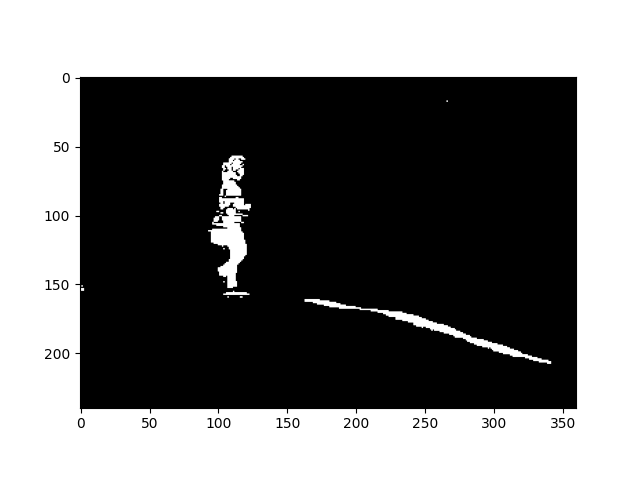
\includegraphics[width=\textwidth]{pedestrian_fg_frame_100.png}
        \caption{Foreground mask}
    \end{subfigure}
    \caption{Comparison of the true image, the motion mask, and the foreground mask for the pedestrian example at frame $100$.}\label{fig:pedestrian-frame-100}
\end{figure}

\subsection{Detection of Moving Canoe}\label{subsec:canoe} % MARK: CANOE

The canoe dataset obtained from \href{changedetection.net}{changedetection.net} shows a section of a river and trees with a canoe passing in front of the camera. In contrast to the pedestrian problem of Subsection~\ref{subsec:pedestrians}, this video possesses a noisy background due to reflections and changes in shade of both the river and the trees. Additionally, most of the frame consists of dark green and brown tones, which means that the greyscaled frames do not exhibit large differences between foreground and background objects.

We repeat the same process as in the pedestrian example of Subsection~\ref{subsec:pedestrians} for the memory sizes $\ell_\text{mem} \in \set{5, 10, 15, 20}$. In this case we need to choose the tolerances for foreground detection in a more careful manner because the video is much more noisy due to reflections on the river. This can be seen in the much less significant difference in minimal residuals in Figure~\ref{fig:canoe-exp-residual}. After experimentation we decided to use the tolerances $\rho \in \set{8 \cdot 10^{-2}, 4.4 \cdot 10^{-2}, 2.8 \cdot 10^{-2}, 2.1 \cdot 10^{-2}}$ for thresholding the minimal residuals.

\begin{figure}[!ht]
    \centering
    \begin{tikzpicture}
        \pgfplotsset{
            width=16cm,
            height=7cm
        }
        \begin{axis}[
            xmin=0, xmax=386,
            ymin=1e-2, ymax=1.5e-1,
            ymode=log,
            xlabel={Index $i$},
            ylabel={Residual $r_i$},
            legend style={
                at={(0.975, 0.05)},
                anchor=south east,
                legend columns=1,
            }
        ]
            \addplot[color=red, smooth, thick] table[col sep=comma, header=has colnames, x index={0}, y index={1}] {canoe_motion_res.csv}; \addlegendentry{$\ell_\text{mem} = 5$}
            \addplot[color=blue, smooth, thick] table[col sep=comma, header=has colnames, x index={0}, y index={2}] {canoe_motion_res.csv}; \addlegendentry{$\ell_\text{mem} = 10$}
            \addplot[color=orange, smooth, thick] table[col sep=comma, header=has colnames, x index={0}, y index={3}] {canoe_motion_res.csv}; \addlegendentry{$\ell_\text{mem} = 15$}
            \addplot[color=black, smooth, thick] table[col sep=comma, header=has colnames, x index={0}, y index={4}] {canoe_motion_res.csv}; \addlegendentry{$\ell_\text{mem} = 20$}
        \end{axis}
    \end{tikzpicture}
    \caption{Residuals $r_i$ for the canoe dataset for memory sizes $\ell_\text{mem} \in \set{5, 10, 15, 20}$; In colour: residuals as computed during the streaming algorithm.}\label{fig:canoe-exp-residual}
\end{figure}

In the comparison of the motion and foreground masks we once again notice the outline effect of the motion detection algorithm. Unfortunately, both masks also suffer from noise pollution. The increased noise of the river reflections might be mitigated by using a regularized of denoised DMD strategy; however, we did not consider this line of argument further.

\begin{figure}[!ht]
    \centering
    \begin{subfigure}{.3\textwidth}
        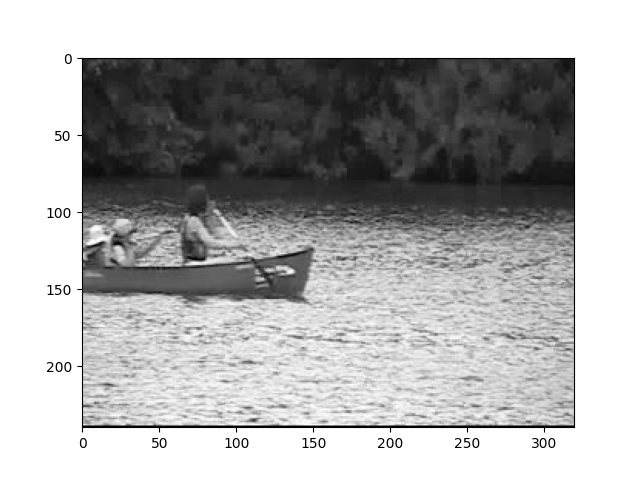
\includegraphics[width=\textwidth]{canoe_frame_100.png}
        \caption{True image}
    \end{subfigure}
    \hfill
    \begin{subfigure}{.3\textwidth}
        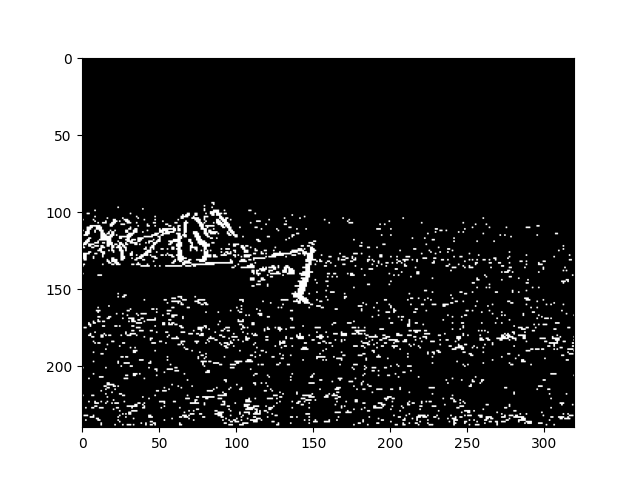
\includegraphics[width=\textwidth]{canoe_motion_frame_100.png}
        \caption{Motion mask}
    \end{subfigure}
    \hfill
    \begin{subfigure}{.3\textwidth}
        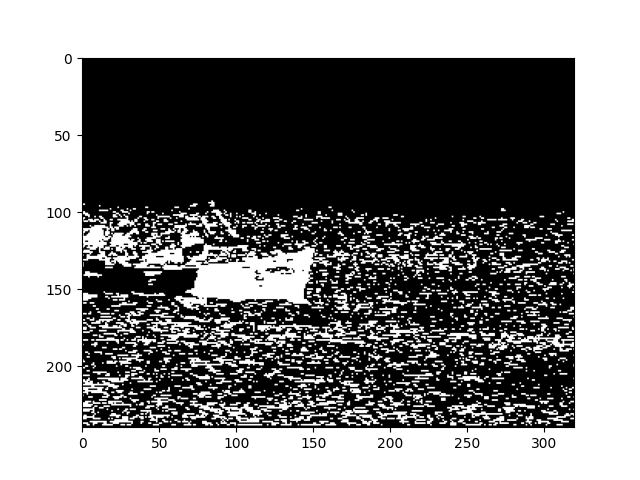
\includegraphics[width=\textwidth]{canoe_fg_frame_100.png}
        \caption{Foreground mask}
    \end{subfigure}
    \caption{Comparison of the true image, the motion mask, and the foreground mask for the canoe example at frame $100$.}\label{fig:canoe-frame-100}
\end{figure}

\subsection{Detection of Sofa}\label{subsec:sofa} % MARK: SOFA

The sofa dataset obtained from \href{changedetection.net}{changedetection.net} shows a sofa around which people move, sit down on the sofa, and handle cardboard boxes. This dataset is useful to consider because some foreground objects become part of the background, for example a box posed in front of the sofa or a person sitting down on the sofa turn into part of the localised background in the streaming DMD algorithm. This is in stark contrast to both previous examples, where the objects were clearly moving and did not stop for extended amounts of time.

This dataset does not have nearly as much noise as the canoe example from Subsection~\ref{subsec:canoe}, which is why we choose the residual tolerances $\rho \in \set{5 \cdot 10^{-3}, 2 \cdot 10^{-3}, 1.5 \cdot 10^{-3}, 10^{-3}}$ for the corresponding memory sizes $\ell_\text{mem} \in \set{5, 10, 15, 20}$.

\begin{figure}[!ht]
    \centering
    \begin{tikzpicture}
        \pgfplotsset{
            width=16cm,
            height=7cm
        }
        \begin{axis}[
            xmin=0, xmax=100,
            ymin=4e-4, ymax=5e-1,
            ymode=log,
            xlabel={Index $i$},
            ylabel={Residual $r_i$},
            legend style={
                at={(0.975, 0.05)},
                anchor=south east,
                legend columns=1,
            }
        ]
            \addplot[color=red, smooth, thick] table[col sep=comma, header=has colnames, x index={0}, y index={1}] {sofa_motion_res.csv}; \addlegendentry{$\ell_\text{mem} = 5$}
            \addplot[color=blue, smooth, thick] table[col sep=comma, header=has colnames, x index={0}, y index={2}] {sofa_motion_res.csv}; \addlegendentry{$\ell_\text{mem} = 10$}
            \addplot[color=orange, smooth, thick] table[col sep=comma, header=has colnames, x index={0}, y index={3}] {sofa_motion_res.csv}; \addlegendentry{$\ell_\text{mem} = 15$}
            \addplot[color=black, smooth, thick] table[col sep=comma, header=has colnames, x index={0}, y index={4}] {sofa_motion_res.csv}; \addlegendentry{$\ell_\text{mem} = 20$}
        \end{axis}
    \end{tikzpicture}
    \caption{Residuals $r_i$ for the sofa dataset for memory sizes $\ell_\text{mem} \in \set{5, 10, 15, 20}$; In colour: residuals as computed during the streaming algorithm.}\label{fig:sofa-exp-residual}
\end{figure}

Similarly to the previous numerical experiments we notice that the motion mask highlights the outlines of moving foreground objects. Importantly, this example also highlights the disadvantages of the dynamic foreground detection algorithm: whenever the foreground objects come to rest the algorithm determines them to be part of the background, hence any prolonged resting may produce faulty results for the supposed foreground. A potential solution to this is to fix the dynamic background once it is established and not update it thereafter; however, this also harbours the downside that the video needs to start with a stationary ``groundtruth'' background, i.e.\ the dynamic algorithm becomes subject to priming in the input data.

\begin{figure}[!ht]
    \centering
    \begin{subfigure}{.3\textwidth}
        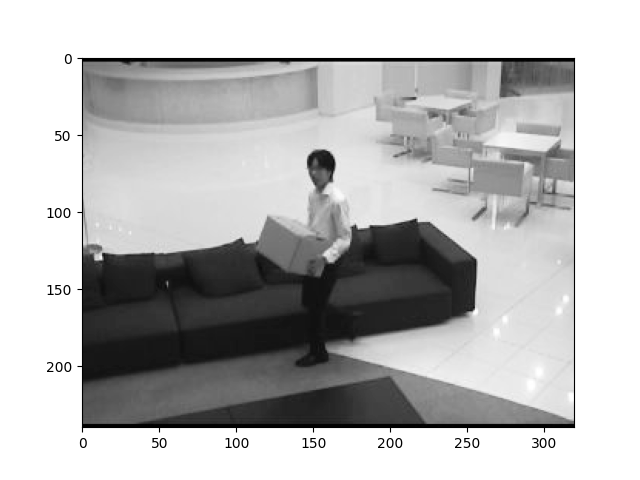
\includegraphics[width=\textwidth]{sofa_frame_100.png}
        \caption{True image}
    \end{subfigure}
    \hfill
    \begin{subfigure}{.3\textwidth}
        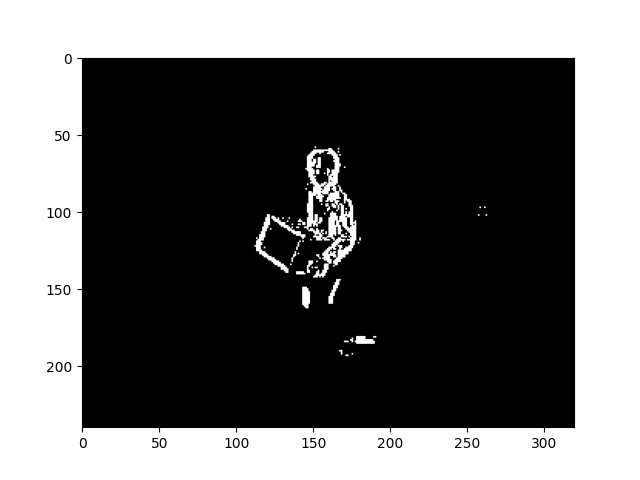
\includegraphics[width=\textwidth]{sofa_motion_frame_100.png}
        \caption{Motion mask}
    \end{subfigure}
    \hfill
    \begin{subfigure}{.3\textwidth}
        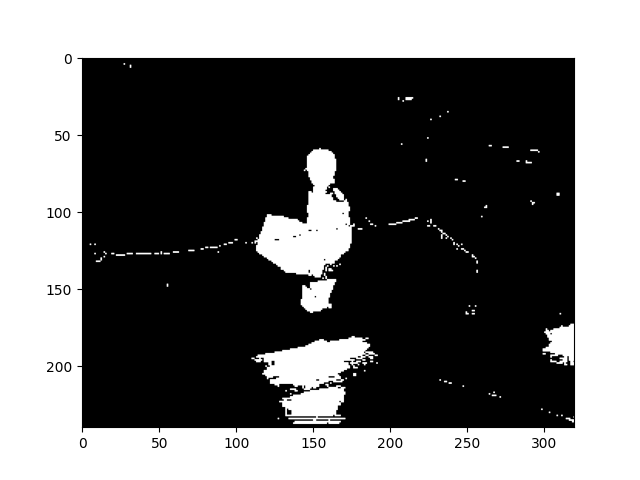
\includegraphics[width=\textwidth]{sofa_fg_frame_100.png}
        \caption{Foreground mask}
    \end{subfigure}
    \caption{Comparison of the true image, the motion mask, and the foreground mask for the sofa example at frame $100$.}\label{fig:sofa-frame-100}
\end{figure}
